\documentclass[a4paper, titlepage]{article}
\usepackage{amsmath}
\usepackage{amsthm}
\usepackage{amssymb}
\usepackage{amsfonts}
\usepackage{graphicx}
\usepackage[left=2cm,right=2cm,bottom=2.5cm,top=2.5cm]{geometry}
\usepackage{fancyhdr}
\usepackage{subcaption}
\usepackage{hyperref}
\usepackage{enumitem}
\usepackage{float}
\usepackage{breqn}
\setlength{\headheight}{14.5pt}

% Theorem-like environments
	\let\oldref\ref
	\renewcommand{\ref}[1]{(\oldref{#1})}
	\newtheorem{theorem}{Theorem}[section]
	\newtheorem{cor}[theorem]{Corollary}
	\newtheorem*{lemma}{Lemma}
	\newtheorem{prop}[theorem]{Proposition}
	\theoremstyle{definition}
	\newtheorem*{note}{Note}
	\newtheorem{defn}[theorem]{Definition}
	\newtheorem{ex}[theorem]{Example}

	\newenvironment{solution}{\renewcommand\qedsymbol{$\square$}\begin{proof}[Solution]}{\end{proof}}


% Set header and footer
%	\pagestyle{fancy}
%	\fancyhf{}

% I like footnotes to be superscript letters rather than numbers
	\renewcommand{\thefootnote}{\alph{footnote}}
	\setlist[enumerate,1]{label={\roman*)}}

%Swap bullets for long dash in itemize
	\renewcommand\labelitemi{---}
	\renewcommand\qedsymbol{\(\blacksquare\)}

% Typesets derivatives nicely using roman d. Adapts size automatically. Stolen from https://tex.stackexchange.com/questions/135944/commath-and-ifinner/135985#135985
% \od{y}{x} is ordinary derivative, \pd{f}{x} is partial derivative. See commath documentation for others
	\usepackage{amsmath}
	\newcommand{\dif}{\mathop{}\!\mathrm{d}}
	\newcommand{\Dif}{\mathop{}\!\mathrm{D}}

	\makeatletter
	\newcommand{\spx}[1]{%
		\if\relax\detokenize{#1}\relax
		\expandafter\@gobble
		\else
		\expandafter\@firstofone
		\fi
		{^{#1}}%
	}
	\makeatother

	\newcommand\pd[3][]{\frac{\partial\spx{#1}#2}{\partial#3\spx{#1}}}
	\newcommand\tpd[3][]{\tfrac{\partial\spx{#1}#2}{\partial#3\spx{#1}}}
	\newcommand\dpd[3][]{\dfrac{\partial\spx{#1}#2}{\partial#3\spx{#1}}}

	\newcommand{\md}[6]{\frac{\partial\spx{#2}#1}{\partial#3\spx{#4}\partial#5\spx{#6}}}
	\newcommand{\tmd}[6]{\tfrac{\partial\spx{#2}#1}{\partial#3\spx{#4}\partial#5\spx{#6}}}
	\newcommand{\dmd}[6]{\dfrac{\partial\spx{#2}#1}{\partial#3\spx{#4}\partial#5\spx{#6}}}

	\newcommand{\od}[3][]{\frac{\dif\spx{#1}#2}{\dif#3\spx{#1}}}
	\newcommand{\tod}[3][]{\tfrac{\dif\spx{#1}#2}{\dif#3\spx{#1}}}
	\newcommand{\dod}[3][]{\dfrac{\dif\spx{#1}#2}{\dif#3\spx{#1}}}

	\newcommand{\genericdel}[4]{%
		\ifcase#3\relax
		\ifx#1.\else#1\fi#4\ifx#2.\else#2\fi\or
		\bigl#1#4\bigr#2\or
		\Bigl#1#4\Bigr#2\or
		\biggl#1#4\biggr#2\or
		\Biggl#1#4\Biggr#2\else
		\left#1#4\right#2\fi
	}
	\newcommand{\del}[2][-1]{\genericdel(){#1}{#2}}
	\newcommand{\set}[2][-1]{\genericdel\{\}{#1}{#2}}
	\let\cbr\set
	\newcommand{\sbr}[2][-1]{\genericdel[]{#1}{#2}}
	\let\intoo\del
	\let\intcc\sbr
	\newcommand{\intoc}[2][-1]{\genericdel(]{#1}{#2}}
	\newcommand{\intco}[2][-1]{\genericdel[){#1}{#2}}
	\newcommand{\eval}[2][-1]{\genericdel.|{#1}{#2}}
	\newcommand{\envert}[2][-1]{\genericdel||{#1}{#2}}
	\let\abs\envert
	\newcommand{\sVert}[1][0]{%
		\ifcase#1\relax
		\rvert\or\bigr|\or\Bigr|\or\biggr|\or\Biggr
		\fi
	}
	\newcommand{\enVert}[2][-1]{\genericdel\|\|{#1}{#2}}
	\let\norm\enVert
	\newcommand{\fullfunction}[5]{%
		\begin{array}{@{}r@{}r@{}c@{}l@{}}
			#1 \colon & #2 & {}\longrightarrow{} & #3 \\
			& #4 & {}\longmapsto{}     & #5
		\end{array}
	}


\title{Langevin MC, \\
  \large or the curse of dimensionality}
\author{B. Han, T.M. Hodgson, M. Holden \& M. Puza}

% Define new commands for typesetting here
\newcommand{\R}{\mathbb{R}}
\renewcommand{\L}{\mathcal{L}}
\renewcommand{\P}{\mathbb{P}}
%\renewcommand{\epsilon}{\varepsilon}
\newcommand{\e}{\mathrm{e}}
\newcommand{\grad}{\nabla}
\newcommand{\E}{\mathbb{E}}



\begin{document}
	\maketitle
	\section*{Abstract}
	\section*{Author Contribution}
	\tableofcontents
	\newpage
	\section{Introduction}
	\documentclass[a4paper]{article}
\usepackage{amsthm}
\usepackage{graphicx}
\usepackage[left=2cm,right=2cm,bottom=2.5cm,top=2.5cm]{geometry}
\usepackage{fancyhdr}
\usepackage{subcaption}
\usepackage{hyperref}
\usepackage{enumitem}

\setlength{\headheight}{14.5pt} 

% Theorem-like environments
	\let\oldref\ref 
	\renewcommand{\ref}[1]{(\oldref{#1})}
	\newtheorem{thm}{Theorem}[section]
	\newtheorem{cor}[thm]{Corollary}
	\newtheorem*{lemma}{Lemma}
	\newtheorem{prop}[thm]{Proposition}
	\theoremstyle{definition}
	\newtheorem*{note}{Note}
	\newtheorem{defn}[thm]{Definition}
	\newtheorem{ex}[thm]{Example}
	
	\newenvironment{solution}{\renewcommand\qedsymbol{$\square$}\begin{proof}[Solution]}{\end{proof}}
	
% Set header and footer
	\pagestyle{fancy}
	\fancyhf{}

% I like footnotes to be superscript letters rather than numbers
	\renewcommand{\thefootnote}{\alph{footnote}}    
	\setlist[enumerate,1]{label={\roman*)}}
	
% Define new commands for typesetting here
	\newcommand{\R}{\mathbb{R}}
	\renewcommand{\L}{\mathcal{L}}  
	\renewcommand{\epsilon}{\varepsilon}
	\newcommand{\e}{\mathrm{e}}

%Swap bullets for long dash in itemize
	\renewcommand\labelitemi{---}
	\renewcommand\qedsymbol{\(\blacksquare\)}

% Typesets derivatives nicely using roman d. Adapts size automatically. Stolen from https://tex.stackexchange.com/questions/135944/commath-and-ifinner/135985#135985
% \od{y}{x} is ordinary derivative, \pd{f}{x} is partial derivative. See commath documentation for others
	\usepackage{amsmath}
	\newcommand{\dif}{\mathop{}\!\mathrm{d}}
	\newcommand{\Dif}{\mathop{}\!\mathrm{D}}
	
	\makeatletter
	\newcommand{\spx}[1]{%
		\if\relax\detokenize{#1}\relax
		\expandafter\@gobble
		\else
		\expandafter\@firstofone
		\fi
		{^{#1}}%
	}
	\makeatother
	
	\newcommand\pd[3][]{\frac{\partial\spx{#1}#2}{\partial#3\spx{#1}}}
	\newcommand\tpd[3][]{\tfrac{\partial\spx{#1}#2}{\partial#3\spx{#1}}}
	\newcommand\dpd[3][]{\dfrac{\partial\spx{#1}#2}{\partial#3\spx{#1}}}
	
	\newcommand{\md}[6]{\frac{\partial\spx{#2}#1}{\partial#3\spx{#4}\partial#5\spx{#6}}}
	\newcommand{\tmd}[6]{\tfrac{\partial\spx{#2}#1}{\partial#3\spx{#4}\partial#5\spx{#6}}}
	\newcommand{\dmd}[6]{\dfrac{\partial\spx{#2}#1}{\partial#3\spx{#4}\partial#5\spx{#6}}}
	
	\newcommand{\od}[3][]{\frac{\dif\spx{#1}#2}{\dif#3\spx{#1}}}
	\newcommand{\tod}[3][]{\tfrac{\dif\spx{#1}#2}{\dif#3\spx{#1}}}
	\newcommand{\dod}[3][]{\dfrac{\dif\spx{#1}#2}{\dif#3\spx{#1}}}
	
	\newcommand{\genericdel}[4]{%
		\ifcase#3\relax
		\ifx#1.\else#1\fi#4\ifx#2.\else#2\fi\or
		\bigl#1#4\bigr#2\or
		\Bigl#1#4\Bigr#2\or
		\biggl#1#4\biggr#2\or
		\Biggl#1#4\Biggr#2\else
		\left#1#4\right#2\fi
	}
	\newcommand{\del}[2][-1]{\genericdel(){#1}{#2}}
	\newcommand{\set}[2][-1]{\genericdel\{\}{#1}{#2}}
	\let\cbr\set
	\newcommand{\sbr}[2][-1]{\genericdel[]{#1}{#2}}
	\let\intoo\del
	\let\intcc\sbr
	\newcommand{\intoc}[2][-1]{\genericdel(]{#1}{#2}}
	\newcommand{\intco}[2][-1]{\genericdel[){#1}{#2}}
	\newcommand{\eval}[2][-1]{\genericdel.|{#1}{#2}}
	\newcommand{\envert}[2][-1]{\genericdel||{#1}{#2}}
	\let\abs\envert
	\newcommand{\sVert}[1][0]{%
		\ifcase#1\relax
		\rvert\or\bigr|\or\Bigr|\or\biggr|\or\Biggr
		\fi
	}
	\newcommand{\enVert}[2][-1]{\genericdel\|\|{#1}{#2}}
	\let\norm\enVert
	\newcommand{\fullfunction}[5]{%
		\begin{array}{@{}r@{}r@{}c@{}l@{}}
			#1 \colon & #2 & {}\longrightarrow{} & #3 \\
			& #4 & {}\longmapsto{}     & #5
		\end{array}
	}
\title{Langevin Monte Carlo, \\
  \large or the curse of dimensionality}
\author{B. Han, T.M. Hodgson, M. Holden \& M. Puza}
\usepackage{palatino}
\begin{document}
	\maketitle 

	\section{Introduction}
	Markov chain Monte Carlo (MCMC) methods are a family of algorithms for calculating numerical approximations of integrals, with applications in computational physics, biology and statistics.  
	
	\subsection*{Monte Carlo Integration}
	Th
		
	
	


		\bibliography{langevinMC.bib}
		\bibliographystyle{plain}
		
\end{document}

	
	\section{Langevin Monte Carlo Algorithms}
	The Langevin equation is a stochastic differential equation (SDE) originally developed to model the movement of a Brownian particle 	\cite{Langevin1908}. The form of interest here is the \emph{overdamped} Langevin equation, in which the particle experiences no average acceleration. The equation is thus
	\begin{equation} \dif X_t = -\nabla U(X_t)\dif t +\sqrt{2}\dif W_t. \label{eq:ODLang}\end{equation}
Here, \(W_t\) is a \(d\)-dimensional Wiener process (Brownian motion) and \(U:\R^d \to \R\) is the potential function. The equation can be thought of as modelling a particle in a potential well with shape \(U\). As each particle moves randomly, it is natural to ask what is the average position of many particles in such a well? It can be shown that in fact the position of a particle moving according to the above dynamics is exactly \(\pi\) +++Reference to earlier subsection/first mention of distribution+++. For a diffusion process this is called the \emph{stationary distribution}\footnote{Another common term is \emph{invariant measure} +++} To show that \(\pi\) is indeed the stationary distribution the following lemma

\begin{lemma}
	For a one-dimensional It\^o diffusion +++add conditions on diffusion/drift+++,
	\[\dif X_t = \mu(X_t)\dif t + \sigma^2(X_t)dW_t,\]
	the Fokker-Planck operator, \(\L^*\), is
	\[\L^*:= -\partial_x(\mu(x)\cdot)+\frac{1}{2}\partial^2_x(\sigma^2(x)\cdot).\]
	A measure \(\pi\) is invariant for the diffusion if and only if
	\[\L^*\pi = 0\]
\end{lemma}
The proof of this is omitted however it can be seen by forming the Fokker-Planck equation for the probability density of the diffusion. The proof that \(\pi\) is the stationary measure of Equation \eqref{eq:ODLang} is given only in the one dimensional case, however it is extendable to higher dimensions. For the Langevin equation, the Fokker-Planck operator is

\[\L^* = \partial_x(U'(x)\cdot)+\partial_{xx}\cdot . \]
So it remains to calculate \(\L^*\pi\).
\begin{align*}
\L^*\pi &= \pd{}{x}\bigg\lbrack U'(x)\pi(x) + \pd{}{x}\pi(x)\bigg\rbrack\\
		&= \pd{}{x}\bigg\lbrack U'(x)\mathcal{Z}\e^{-U(x)}+ \left(-U'(x)\mathcal{Z}\e^{-U(x)}\right)\bigg\rbrack\\
		&= \pd{}{x}\lbrack 0 \rbrack\\
		&= 0
\end{align*}
Hence \(\pi\) is indeed the invariant measure of \eqref{eq:ODLang}. \qed
\\
\\
Although this shows that the Langevin equation has an invariant measure, the question of convergence to this measure remains unanswered. Roberts and Tweedie give the following restriction \cite{RT96}.
\begin{theorem}[Theorem 2.1, \cite{RT96}]
	Let \(P^t_X(x,A) = \P(X_t\in A | X_0 =x_0)\) and suppose that \(\grad U(x)\) is continuously differentiable and that, for some \(N,a,b < \infty\),
	\[\grad U(x)\cdot x \leq a|x|^2 + b, \qquad |x|>N. \]
	Then the measure \(\pi\) is invariant for the Langevin diffusion \(X\). Moreover, for all \(x \in \R^d \) and Borel sets \(A\),
	\[\|P^t_X(x,\cdot) - \pi \| = \frac{1}{2}\sup_A \big|P^t_X(x,A)-\pi(A)\big| \to 0\]

\end{theorem}
+++Should this norm be an integral? Add exponentially fast convergence/spectral gap inequality? Figure of \(U=x^2/2\)? 2d?  +++\\

\begin{figure}[ht]
	\centering
		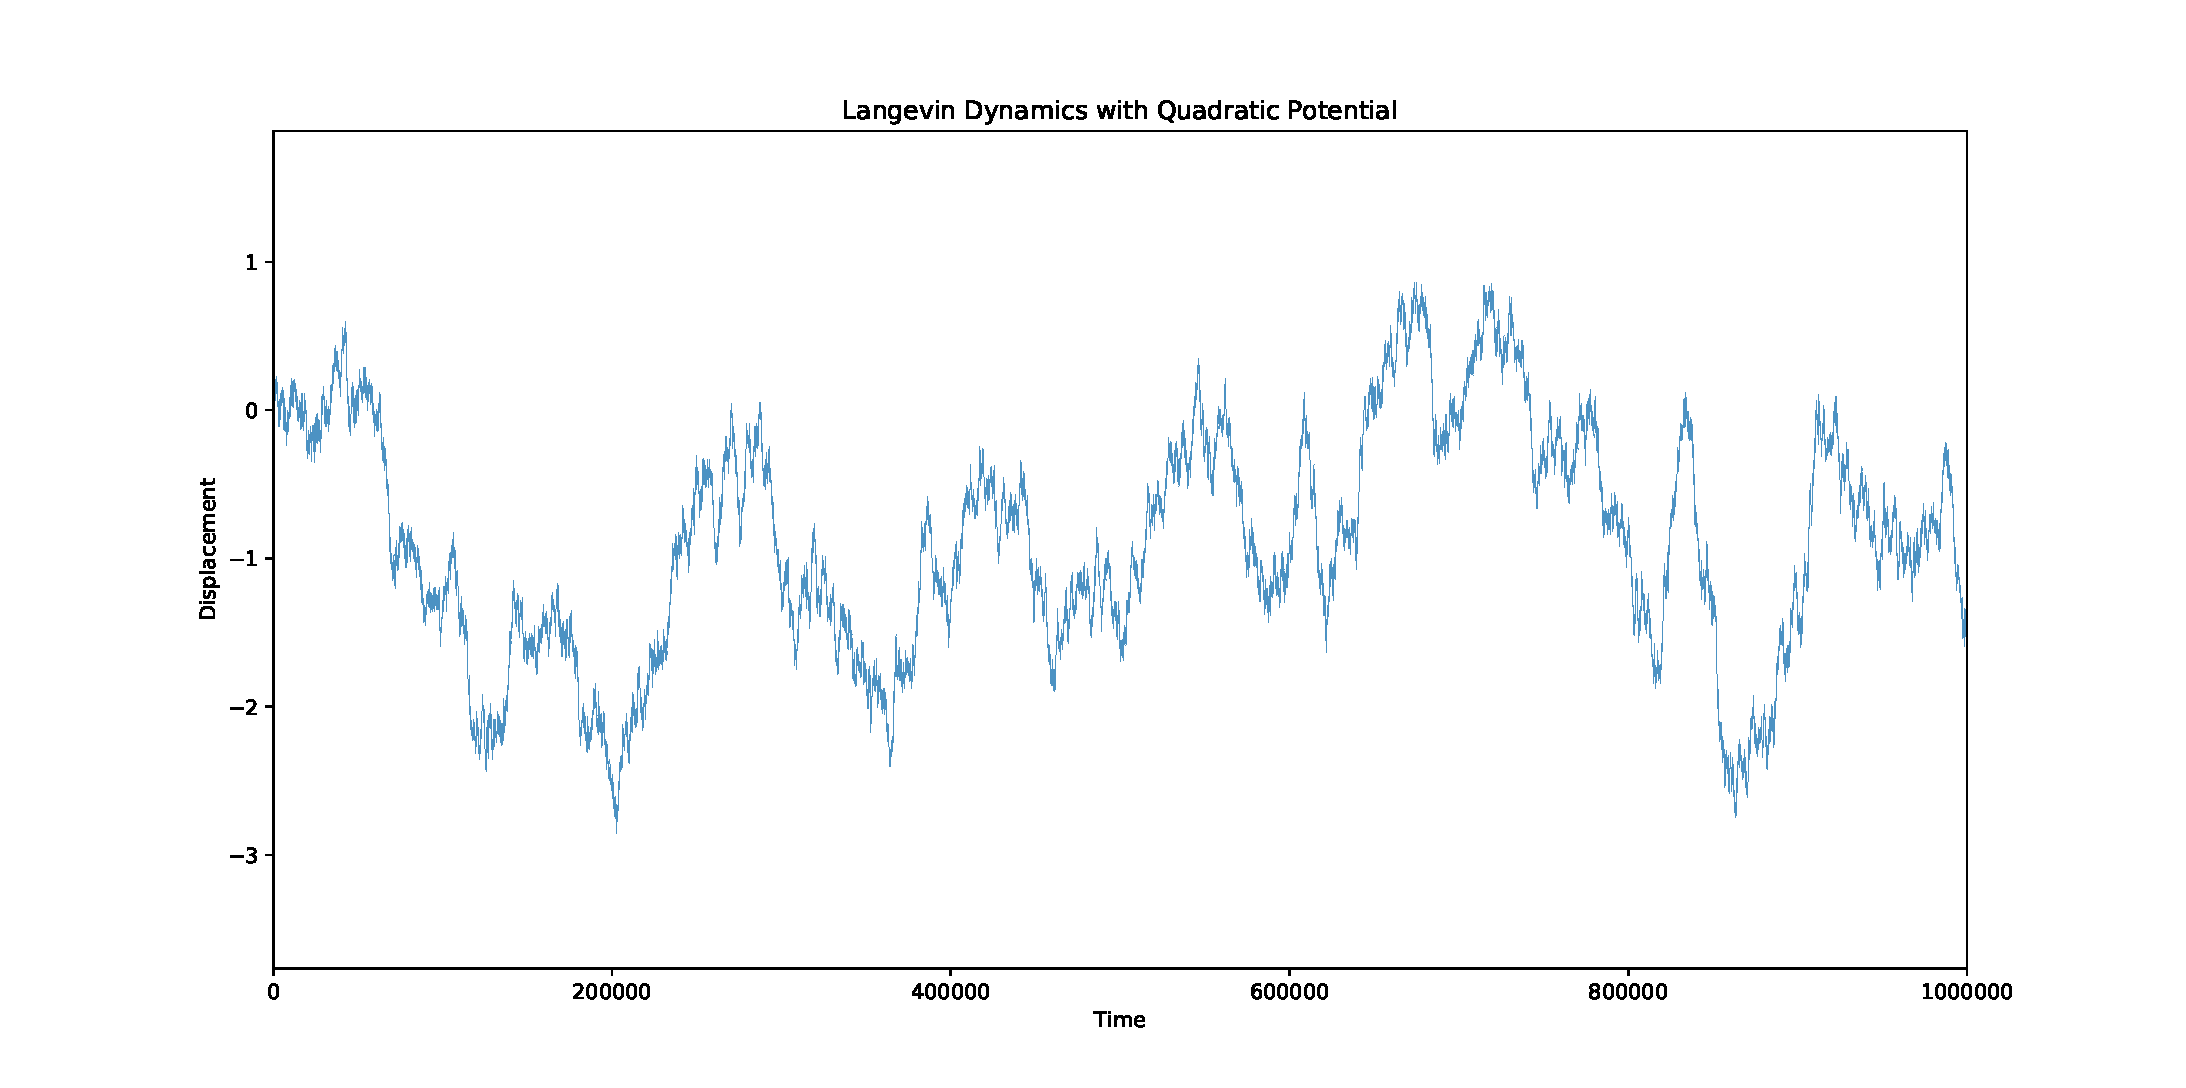
\includegraphics[width=\linewidth]{quadraticLD.pdf}
	\caption{Simulating Langevin dynamics in one dimension with a quadratic potential \(U(x)=x^2/2\)}
	\label{fig:quadLD}
\end{figure}

The problem of sampling from the high dimensional distribution has been reduced to being able to accurately simulate Langevin dynamics. However, this is not as simple as it sounds. To simulate the continuous process  \eqref{eq:ODLang}, it must first be discretised. However, doing so may not preserve the convergence to the invariant measure. The discretised process may not have the same stationary measure or it may not even exist. This means that the method used to discretise must be chosen carefully to ensure good convergence properties. The most natural way to discretise an SDE is to use the stochastic analogue of the (forward) Euler method used on ordinary differential equations, known as the Euler-Maruyama (EM) method. Doing so leads to the Unadjusted Langevin Algorithm (\texttt{ULA}).

\subsection{The Unadjusted Langevin Algorithm}
Applying the Euler-Maruyama method to Equation \eqref{eq:ODLang} gives the following iterative scheme.

\[X_{n+1} = X_n -h \nabla U(X_n) +\sqrt{2h} Z_{n+1},\qquad X_0= x_0 \]
Here the \(Z_n \) are i.i.d. standard normal random variables and \(h\) is the step size. This is equivalent to \(X_{n+1} \sim N(X_n - h\grad U(X_n), 2h I_d )\).\footnote{\(I_d\) denotes the \(d \times d\) identity matrix.} A simple example shows that this discretisation does not converge to \(\pi\). Let \(\pi\) be a standard Gaussian distribution, that is \(U(x) = |x|^2/2 \) and choose \(h = 1\). Then the update is given by

\begin{align*}
	X_{n+1} &\sim N(X_n - \grad U(X_n), 2)\\
	& \sim  N(X_n - X_n, 2)\\
	& \sim N(0,2) \nsim \pi .
\end{align*}
So the chain converges immediately, but to the wrong distribution. Let \(\pi^{\text{ULA}}_{h} \) denote the stationary distribution of \texttt{ULA} with a stepsize \(h\). This is not the only issue that can occur. As well as not converging to the correct distribution, the discretised chain may not be  ergodic, even when the continuous diffusion is exponentially ergodic \cite{RT96}. In particular, the algorithm misbehaves when the gradient of the potential is superlinear. That is,
\[\liminf_{\|x\|\to \infty} \frac{\|\grad U(x)\|}{\|x\|} = +\infty. \]
To mitigate these issues there are two main approaches: taming the gradient and Metropolisation. A further third method involves using a different discretisation scheme.  Our main focus will be the former, although all three approaches will be discussed.

\subsection{MALA}
Before describing the Metropolis-adjusted Langevin algorithm \texttt{MALA}, it is pertinent at this point to recall the random walk Metropolis-Hastings algorithm \texttt{RWM }\cite{Hastings70, Metropolis53}. This popular variant of the Metropolis-Hastings algorithm \emph{proposes} values and then accepts/rejects them according to some probability \(\alpha\).  So given \(X_n\), propose a candidate \(Y_{n+1}\) as
\[Y_{n+1} = X_n + \sqrt{2h} Z_{n+1}.\]
Once again, \(h\) is the stepsize and \(Z\) is a normal random variable. Then, accept or reject this proposal using Metropolis rejection, that is with some probability
\[\alpha(X_n,Y_{n+1}) = 1\wedge \frac{\pi(Y_{n+1})q(Y_{n+1},X_n)}{\pi(X_n)q(X_n,Y_{n+1})}.\footnote{Here \(t\wedge s = \min\lbrace t,s\rbrace.\) }\]
Here \(q(x,y)\) is the transition probability, \(\P(Y_{n+1}=y | X_{n}=x)\sim N(X_n, h^2)\). This rejection step is key in creating a kernel that is reversible and thus invariant for the measure \(\pi\). \\


\texttt{MALA} can be seen as another variant of the Metropolis-Hastings algorithm, using Langevin dynamics to propose new states. It is perhaps better understood as \texttt{ULA} but with an added Metropolis rejection step \cite{RT96}. Adding this rejection step means the algorithm always has the correct invariant distribution, although convergence is still not guaranteed as the following theorem shows.

\begin{theorem}[Theroem 4.2, \cite{RT96}]
	If \(\pi\) is bounded, and
		\[\liminf_{\|x\|\to \infty} \frac{\|\grad U(x)\|}{\|x\|} > \frac{4}{h}\]
	then the \texttt{MALA} chain is not exponentially ergodic. +++define exp ergodic+++
\end{theorem}
So it can be seen that \texttt{MALA} is not without its issues, and does not solve all the problems of \texttt{ULA}. The concept of taming was introduced to try and reduce the magnitude of these problems.

\subsection{Taming the Gradient}
We have seen that both \texttt{ULA} and \texttt{MALA} run into issues when the gradient of the potential is superlinear. Given an SDE such as \eqref{eq:ODLang}, taming adjusts the drift coefficient in such a way that preserves the invariant measure and improves speed of convergence \cite{Brosse18tULA,RT96,Sabanis13}. To do this, a family of drift functions \((G_h)_{h>0}, \ G_h:\R^d \to \R^d\) are introduced. The SDE to be discretised is thus
	\begin{equation*} \dif X_t = -G_h(X_t)\dif t +\sqrt{2}\dif W_t. \end{equation*}
Applying the Euler-Maruyama method gives the following Markov chain
	\[X_{k+1} =X_k-hG_h(X_k)+\sqrt{2h}Z_{k+1},\qquad  X_0=x_0.\]
To preserve the invariant measure, some restrictions must be placed on \((G_h)_{h>0}\), namely that they are `close' to \(\grad U\) ({\bf A1}) while {\bf A2} ensures ergodicity is preserved and improves stability \cite{Brosse18tULA}. 

\begin{enumerate}[label={\bf A{\arabic*}}]
	\item  For all \(h>0, G_h\) is continuous. There exist \(\alpha\geq 0, C_{\alpha}<+\infty\) such that for all \(h >0 \) and \(x \in \R^d\),
		\[\|G_h(x)-\grad U(x)\| \leq hC_{\alpha}(1+\|x\|^{\alpha}).\]\label{A1}
	\item For all \(h>0\),
		\[ \liminf_{\|x\|\to \infty} \bigg\lbrack \bigg\langle \frac{x}{\|x\|}, G_h(x)\bigg\rangle - \frac{h}{2\|x\|}\|G_h(x)\|^2\bigg\rbrack >0\]\label{A2}
\end{enumerate}
Here we consider two specific taming functions,
 \begin{align*}
 T_h(x) = \frac{\grad U(x)}{1+h\|\grad U(x)\|}, &&  T^{\text{\sc \tiny RT}}_h = \frac{\grad U(x)}{1\vee h\|\grad U(x)\|}.
 \end{align*}
Brosse et al. introduced and studied \(T_h\) whilst Roberts \& Tweedie suggested \(T^{\text{\sc \tiny RT}}_h\), later analysed by Bou-Rabee \& Vanden-Eijnden \cite{BV10MALTA,Brosse18tULA,RT96}. Both taming functions retain the direction of the gradient, only reducing the magnitude of its effect. The latter is the usual \texttt{ULA} until the gradient gets large enough \((\|\grad U(x)\|> 1/h)\), at which point it begins normalising. In contrast, the first will always tame, regardless of size of the gradient. However for the scaling to have noticeable effect, the gradient must be \(\mathcal{O}(h^{-1})\).
When \(T_h\) is the taming function, the algorithm will be referred to as \texttt{tULA}, the tamed unadjusted Langevin algorithm. When the second is applied, it will be called \texttt{MALTA}, the Metropolis adjusted Langevin truncated algorithm after \cite{RT96}. Any tamed algorithm using \(T_h\) will be prefixed with a lowercase \texttt{t}. For a proof that \(T_h\) satisfies \ref{A1} and \ref{A2}, see \cite[Lemma~2]{Brosse18tULA}.
\\
When the problem is ill-conditioned, taming the gradient does not help +++Kostas' example, ill-cond Gauss does this motivate coordinatewise?+++. 
\subsubsection{tULA/c}
So far, the gradient has only been tamed globally. This has a negative side effect in that it heavily restricts movement in all dimensions, regardless of whether the gradient is superlinear in that direction. A solution to this is to use coordinatewise taming with the following drift.
  \[T^c_{h}(x) =\left(\frac{\partial_i U(x)}{1+h|\partial_i U(x)|}\right)_{i=\lbrace 1, \dots, d\rbrace} \]
This allows each dimension to be scaled individually. Any algorithm with coordinate-wise taming will be suffixed with a lowercase \texttt{c}.

\subsection{Discretise Differently}
An alternative approach is to use a different discretisation of the SDE \eqref{eq:ODLang}, which we consider in this section. The first is an extension of the Euler method \cite{Sabanis18tHOLA}, while the latter uses a non-Markovian scheme developed for use in molecular dynamics \cite{LM12}.
\subsubsection{Higher Order Langevin Algorithm}
As in the ordinary case, the Euler-Maruyama method is not the only way of discretising an SDE. One can also take a higher order expansion, analagous to the Runge-Kutta method, known as the order 1.5 Wagner-Platen expansion\footnote{Or the stochastic Runge-Kutta method \cite{Schaffter10numericalintegration}}. For a one dimensional Langevin diffusion \eqref{eq:ODLang}, this is 
\[X_{n+1} = X_n -hU'(X_n)+\sqrt{2h}Z_n -\sqrt{2} U''(X_n) \tilde{Z}_n +\frac{ h^2 }{2}\bigg\lbrack U'(X_n)U''(X_n)-U'''(X_n)\bigg\rbrack.  \]
Here, \(\tilde{Z}_n\) is defined as
\[  \tilde{Z}_n = \int_{t_n}^{t_{n+1}} \int_{t_n}^s \dif W_r \dif s. \]
This is a \(d\)-dimensional Gaussian random variable with mean \(0_d\) and covariance \(\frac{1}{3}h^3 I_d\). 
Use an It\^o-Taylor expansion
\[X_{n+1} = X_n + \mu_{h}(X_n)h +\sigma_{h}(X_n)\sqrt{h}Z_{n+1}\]
where
\[\mu_{h}(x) = -\grad U_{h}(x) +\frac{h}{2}\left( \left( \grad^2U\grad U\right)_{h}(x) - \vec{\Delta}(\grad U)_{h}(x)\right) ,\]
and \(\sigma_{h}(x) = \text{diag}\left(\left( \sigma_{h}^{(k)}(x)\right)_{k\in \lbrace 1,\dots,d\rbrace}\right)\) with,
\[\sigma_{h}^{(k)}(x) = \sqrt{2+\frac{2h^2}{3}\sum_{j=1}^d |\grad^2 U_{h}^{(k,j)}(x)|^2 - 2h \grad^2 U_{h}^{(k,k)}(x)}\]
ALSO need to define the h subscript, i.e. the tamed variables.  Although fn depends on gamma it doesn't indicate that taming has occurred.
\subsubsection{LM}
\cite{LM12}
Non-Markovian scheme,
\[X_{n+1} = X_n +h \grad U(X_n) + \sqrt{\frac{h}{2}} \left(Z_n + Z_{n+1}\right) \]


\subsection{Other Methods}
\subsubsection{RWM}
Popular variant of the Metropolis-Hastings algorithm (CITE) with a normal proposal.
\[U_{n+1} = X_n + \sqrt{2h} Z_{n+1}\]

Calculate acceptance probability
\[\alpha(X_n,U_{n+1}) = 1\wedge \frac{\pi(U_{n+1})q(U_{n+1},X_n)}{\pi(X_n)q(X_n,U_{n+1})}\]
Here \(q(x,y)\) is the transition probability, \(\P(X_{n+1}=y | X_{n}=x)\). If \texttt{rand}\(\leq\alpha\),
\[X_{n+1} = U_{n+1}.\]
That is,
\[X_{n+1} = \mathbb{I}(u\leq \alpha)U_{n+1} +\mathbb{I}(u > \alpha)X_n \]

\subsection{Visualization}
A demonstration of the above methods has been implemented using the visualization library of \cite{rogozhnikov2016hmc}\footnote{With kind permission of Alex Rogozhnikov, \url{https://arogozhnikov.github.io/about/}.}. The visualization dynamically follows the trace of a chosen method applied to a chosen two-dimensional distribution. Distributions of various qualitative properties are available. This can be found at the following \textsc{url}: \\

   \centerline{ \url{http://goatleaps.xyz/assets/ULA/ULA.html}}

\begin{figure}[H]
\centering
  \begin{minipage}[b]{0.8\textwidth}
  \centering
    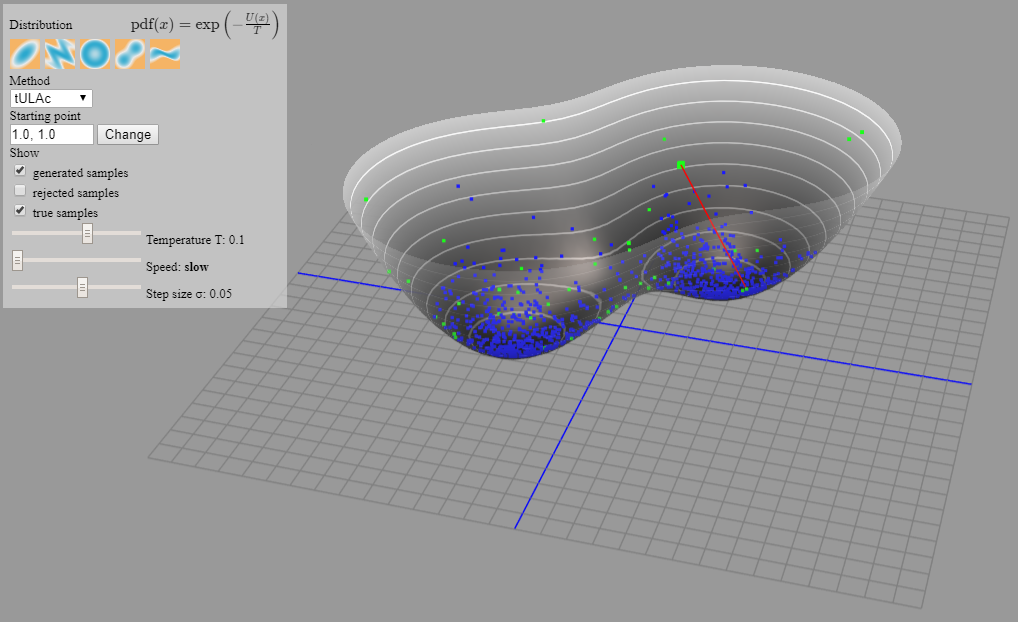
\includegraphics[width=0.8\textwidth]{Figures/ulavis.PNG}
    \caption{Screenshot from the visualization;  tULAc applied to a Gaussian mixture distribution.}
  \end{minipage}
\end{figure}

	\section{Beyond Moments}
	While first and second moments give us some idea of the performance of our sampling algorithms, we ideally would like a fuller picture.  In this section we compare the performance of algorithms using the total variation distance, $L^2$-Wasserstein distance and Kullback--Leibler divergence.  Using these measures, we can compare the performance to theoretical upper bounds for \texttt{ULA}.

\subsection{Statistical Distances}
Let $\mathcal{B}(\R^d)$ denote the Borel $\sigma$-algebra on $\R^d$. Let $P$ and $Q$ be probability measures on the space $(\R^d, \mathcal{B}(\R^d))$.  Then we define the total variation distance, Kullback--Leibler divergence and Wasserstein metric as follows:

\begin{defn}[Total Variation]
The total variation distance between two probability measures $P$ and $Q$ on $(\Omega, \mathcal{F})$ is defined as
$$
\norm{P - Q}_{TV} = \sup_{A \in \mathcal{F}} \abs{P(A) - Q(A)}.
$$
\end{defn}
\begin{prop}
If the set $\Omega$ is countable then this is equivalent to half the $L^1$ norm.
$$
\norm{P - Q}_{TV} = \frac{1}{2} \norm{P-Q}_1 = \frac{1}{2} \sum_{\omega \in \Omega} \abs{P(\omega) - Q(\omega)}
$$
\end{prop}
\begin{proof}
Let $B = \{\omega: P(\omega) \geq Q(\omega)\}$ and let $A \in \mathcal{F}$ be any event.  Then
$$
P(A) - Q(A) \leq P(A \cap B) - Q(A \cap B) \leq P(B) - Q(B).
$$
The first inequality holds since $P(\omega)-Q(\omega) < 0$ for any $\omega \in A \cap B^c$, and so the difference in probability cannot be greater if these elements are excluded.  For the second inequality, we observe that including further elements of $B$ cannot decrease the difference in probability.
Similarly,
$$
Q(A) - P(A) \leq Q(B^c) - P(B^c) = P(B) - Q(B)
$$
Thus, setting $A=B$, we have that $\abs{P(A)-Q(A)}$ is equal to the upper bound in the total variation distance.  Hence,
$$
\norm{P-Q}_{TV} = \frac{1}{2} \abs{P(B)-Q(B)+Q(B^c)-P(B^c)} = \frac{1}{2} \sum_{\omega \in \Omega} \abs{P(x)-Q(x)}
$$
\end{proof}


\textbf{POSSIBLY TAKE OUT KL DIVERGENCE??}


\begin{defn}[Kullback--Leibler Divergence]
Let $P$ and $Q$ be two probability measures on $(\Omega, \mathcal{F})$.  If $P \ll Q$, the Kullback--Leibler divergence of $P$ with respect to $Q$ is defined as
$$
KL(P|Q) = \int_\Omega \frac{d P}{d Q} log \left(  \frac{d P}{d Q} \right) d Q.
$$
\end{defn}

\textbf{LITTLE MORE INTUITION ON WASSE??}

Finally we consider the Wasserstein distance.  If $P$ and $Q$ are probability measures on $(\R^d,\mathcal{B}(\R^d)$, we say that $\gamma$ is a transport plan between two probability measures $P$ and $Q$ if it is a probability measure on $(\R^d \times \R^d, \mathcal{B}(\R^d \times \R^d))$ such that for any Borel set $A \subset \R^d$, $\gamma(A \times \R^d)=P(A)$ and $\gamma(\R^d \times A) = Q(A)$.  We denote the set of all such transport plans by $\Pi(P,Q)$.

\begin{defn}[Wasserstein distance]
For two probability measures, $P$ and $Q$, the $L^p$-Wasserstein distance is given by
$$
W_p(P,Q) = \left( \inf_{\gamma \in \Pi(P,Q)} \int_{\R^d \times \R^d} \norm{x-y}^p d \gamma(x,y) \right)^{1/p}.
$$
\end{defn}

We will restrict our attention mainly to $L^1$-Wasserstein and $L^2$-Wasserstein distances. Due to practical impossibility of computing higher-dimensional Wasserstein distances, we also introduce a compuatationally more feasible variant, the Sliced Wasserstein distance. First proposed in \cite{rabin2011wasserstein} and further elaborated on, for example, in \cite{gswd}, the Sliced Wasserstein distance exploits the fact that the Wasserstein distance between 1-dimensional probability measures $P, Q$ can be computed with an explicit formula $\abs{F^{-1}(t)-G^{-1}(t)}^p dt$ where $F$ and $G$ are the CDFs of $P$ and $Q$ respectively \cite{ramdas2017wasserstein}.


\begin{defn}[Sliced Wasserstein distance]
For two probability measures, $P$ and $Q$, the $L^p$-Wasserstein distance is given by
$$
SW_p(P,Q) = \left( \inf_{\gamma \in \Pi(P,Q)} \int_{\R^d \times \R^d} \norm{x-y}^p d \gamma(x,y) \right)^{1/p}.
$$
\end{defn}

The main reason why we can use the Sliced Wasserstein distance as an approximation to the Wasserstein distance is the following inequality, proved in asdfasdfasd 


\subsection{Theoretical Non-asymptotic Error Bounds}
Theoretical bounds on the total variation distance between the distribution of the $n^\text{th}$ iterate of the unadjusted Langevin Algorithm were first provided in the case of a `warm start' in \cite{dalalyan2017theoretical}.  Then \cite{durmus2016high}, \cite{durmus2017nonasymptotic} improve and consider Wasserstein distance.  These papers showed that $O(d/\epsilon)$ iterations are needed for precision level $\epsilon$.

\texttt{ULA} \cite{dalalyan2019user}
\texttt{tULA} \cite{Brosse18tULA}
\texttt{HOLA} \cite{Sabanis18tHOLA}
\texttt{MALA} \cite{bou2013nonasymptotic}



\section{Implementation}
\subsection{Constructing Histograms}
\subsection{Comparing continuous and discrete distributions}
\subsubsection{Sliced Wasserstein}




    \section{Future Work: SGLD}
    % \documentclass[a4paper]{article}

% \usepackage[english]{babel}
% \usepackage[utf8]{inputenc}
% \usepackage{amsmath}
% \usepackage{graphicx}
% \usepackage[colorinlistoftodos]{todonotes}
% \usepackage{titling}
% \usepackage[margin=40mm]{geometry}
% \usepackage{tikz}
% \usepackage{lipsum}
% \usepackage{amsfonts}
% \usepackage{amsmath,amssymb}
% \usepackage{breqn}

% \newtheorem{theorem}{Theorem}


% \newtheorem{lemma}[theorem]{Lemma}
% \newtheorem{corollary}{Corollary}[theorem]



% \begin{document}
% \setlength{\droptitle}{-0.5in}


\normalsize
\textbf{Stochastic Gradient Langevin Dynamics}\\
In this section, we will closely follow\cite{pitfalls}



\subsection{Introduction}

Normally, samples in machine learning are of huge sample sizes, for which most MCMC algorithms are not designed to process. 
As a result of the computational cost, several new approaches were proposed recently, Stochastic Gradient Langevin Dynamics (SGLD) is a popular one. 
SGLD is based on the Langevin Monte Carlo (LMC)
LMC – a discretization of a continuous-time process, it requires to compute the gradient of the log-posterior at the current fit of the parameter and avoid the accept/reject step.
SGLD – use unbiased estimator of the gradient of log-posterior based on subsampling, suitable for samples of huge size. 


\subsection{Governing Equation}

Langevin Stochastic Differential Equation (SDE):$$d\theta_t = -\nabla U(\theta_t)d +\sqrt{2}d B_t$$ where $(B_t)_{t \geq 0}$ is a d-dimensional Brownian motion. 

Euler discretization of the Langevin SDE:
$$\theta_{k+1} = \theta_k - \gamma \nabla U(\theta_k)+\sqrt{2\gamma} Z_{k+1}$$, where $\gamma > 0$ is a constant step size and $(Z_k)_{k\geq1}$ is a sequence of i.i.d standard d - dimensional Guassian vectors. 

To reduce the costs of the algorithms, we will switch to SGLD, for which we will replace $\nabla U$ with an unbiased estimate $\nabla U_0+(\frac{N}{p}) \sum_{i\in S}\nabla U_i$, where S is a minibatch of {1,...., N} with replacement of size p. Our iterations were then updated as
$$\theta_{k+1} = \theta_{k}-\gamma \Bigg (\nabla U_0(\theta_k)+\frac{N}{p}\sum_{i\in S_{k+1}}\nabla U_i(\theta_k)\Bigg )+\sqrt{2\gamma}Z_{k+1}$$

Stochastic Gradient Descent (SGD) is characterised by the same recursion as SGLD without the Gaussian noise, (the last term):


$$\theta_{k+1} = \theta_{k}-\gamma \Bigg (\nabla U_0(\theta_k)+\frac{N}{p}\sum_{i\in S_{k+1}}\nabla U_i(\theta_k)\Bigg)$$

\subsection{Analysis in Wasserstein distance}
\subsection{Definitions and Notations in Markov chain theory}
$\mathcal{P}_2(\mathbb{R}^d)$ the set of probablity measures with finite second momet.\\
$\mathcal{B}(\mathbb{R}^d)$ the Borel $\sigma$ - algebra of $\mathbb{R}^d$.\\
For $\lambda, \nu \in \mathcal{P}_2(\mathbb{R}^d)$, we define the Wasserstein distance by 

$$W_2(\lambda, \nu) =\inf_{\xi \in \Pi(\lambda, \nu)}(\int_{\mathbb{\mathbb{R}^d \times \mathbb{R}^d}}||\theta-\vartheta)||^2 \xi(d\theta, d\vartheta))^{\frac{1}{2}}$$
where, $\Pi(\lambda, \nu)$ is the set of probablity measures $\xi$ on $\mathcal{B}(\mathbb{R}^d)\otimes\mathcal{B}(\mathbb{R}^d)$ satisfying for all $A \in \mathcal{B}(\mathbb{R}^d), \xi(A \times \mathbb{R}^d)= \lambda(A)$ and $\xi (\mathbb{R}^d \times A) = \nu(A)$.\\
For any probablity measure $\lambda$ on $\mathcal{B}(\mathbb{R}^d)$, we define $\lambda R$ for all $A \in \mathcal{B}(\mathbb{R}^d)$ by $\lambda R(A) = \int_{\mathbb{R}^d}\lambda(d\theta)R(\theta, A)$.\\
For all $k\in \mathbb{N}*$, we define the Markov kernel $R^k$ recursively by $R^1 = R$ and for all $\theta \in \mathbb{R}^d$ and $A \in \mathcal{B}(\mathbb{R}^d)$, $R^{k+1}(\theta, A) = \int_{\mathbb{R}^d}  R^k(\theta, d\vartheta)R(\vartheta, A).$\\
A probablity measure $\bar{\pi}$ is invariant for R if $\bar{\pi}R = \bar{\pi}$.\\
Our algorithms LMC, SGLD, SGD and SGLDFP algorithms are homogeneous Markov chains with Markov kernels denoted $R_{LMC}, R_{SGLD}, R_{SGD}$ and $R_{FP}$.

\subsection{Results}
For lemma 1, Theorem 2 and Corollary 3, we assume H1, H2 and H3.
\begin{lemma}
For any step size $\gamma \in (0, \frac{2}{L})$, $R_{SGLD}$(respectively $R_{LMC}, R_{SGD}, R_{FP}$) has a unique invariant measure $\pi_{SGLD}\in \mathcal{P}_2(\mathbb{R}^d)$(respectively $\pi_{LMC}, \pi_{SGD}, \pi_{FP}$). In addition, for all $\gamma \in (0, \frac{1}{L}], \theta\in \mathbb{R}^d and k\in\mathbb{N}$,
$$W_2^2(R_{SGLD}^k(\theta, \cdot), \pi_{SGLD})\leq(1-m\gamma)^k\int_{\mathbb{R}^d}||\theta-\vartheta||^2\pi_{SGLD}(d\vartheta)$$
same inequality holds for LMC, SGD and SGLDFP.
\end{lemma}
\begin{theorem}
For all $\gamma\in(0,\frac{1}{L}], \lambda, \nu\in \mathcal{P}_2(\mathbb{R}^d) and n\in\mathbb{N}$, we have the following upper- bounds in Wasserstein distance between
\begin{enumerate}
	\item 
	LMC and SGLDFP,

\begin{dmath}	
W_2^2(\lambda R_{LMC}^n, \nu R_{FP}^n)\leq(1-m\gamma)^nW_2^2(\lambda, \nu) + \frac{2L^2\gamma d}{pm^2}+\frac{L^2\gamma^2}{p}n(1-m\gamma)^{n-1}\int_{\mathbb{R}^d}||\vartheta-\theta*||^2 \mu(d\vartheta)
\end{dmath},
	\item 
	the Langevin diffusion and LMC,
\begin{dmath}
W_2^2(\lambda R_{LMC}^n, \mu P_{n\gamma})\leq2(1-\frac{mL\gamma}{m+L})^nW_2^2(\lambda, \mu)+d\gamma\frac{m+L}{2m}(3+\frac{L}{m})(\frac{13}{6}+\frac{L}{m})\\+ne^{-(\frac{m}{2})\gamma(n-1)}L^3\gamma^3(1+\frac{m+L}{2m})\int_{\mathbb{R}^d}||\vartheta - \theta*||^2 \mu(d\vartheta)
\end{dmath},
	\item 
	SGLD and SGD
	\begin{dmath}
	W_2^2(\lambda R_{SGLD}^n, \mu R_{SGD}^n)\leq (1-m\gamma)^n W_2^2(\lambda, \mu)+\frac{(2d)}{m}.
	\end{dmath}
\end{enumerate}
\end{theorem}
Proof omitted.
\begin{cor}
Set $\gamma - \frac{\eta}{N} with \eta \in (0, \frac{1}{(2L)}]$ and assume that $lim \inf_{N \to \infty}mN^{-1}>0$. Then
\begin{enumerate}
\item
for all $n \in N$, we get $W_2(R_{LMC}^n(\theta*, \cdot), R_{FP}^{n}(\theta*, \cdot)) = \sqrt{d\eta}\mathcal{O}(N^{-\frac{1}{2}})$ and $W_2(\pi_{LMC}, \pi_{FP}) = \sqrt{d\eta}\mathcal{O}(N^{-\frac{1}{2}})$.
\item 
for all $n\in \mathbb{N}, we get W_2(R_{SGLD}^{n}(\theta*, \cdot), R^n_{SGD}(\theta*, \cdot)) = \sqrt{d}\mathcal{O}(N^{-\frac{1}{2}})$, and $W_2(\pi_{SGLD}, \pi_{SGD}) = \sqrt{d}\mathcal{O}(N^{-\frac{1}{2}})$.
\end{enumerate}
\end{cor}



	\bibliography{langevinMC.bib}
	\bibliographystyle{plain}

\end{document}
